\section{Arquitectura del sistema}

El sistema contendr\'a los siguientes m\'odulos:
\begin{description}
\item[Sistema de Mensajer\'ia] Este m\'odulo del sistema ser\'a el encargado de generar informaci\'on de pruebas para posteriormente ser procesada.

\item[Procesamiento de texto] Este m\'odulo tiene como objetivo el recibir un archivo de texto con la conversaci\'on a analizar el cual fue generado en el m\'odulo de mensajer\'ia. La salida de \'este ser\'a una estructura invariante para poder ser analizada.

\item[API de an\'alisis] Ser\'a el módulo que mediante reconocimiento de patrones, har\'a una revisión de los textos para poder clasificar a una fuente en un comportamiento.

\item[M\'odulo integrador]Este m\'odulo es el encargado de presentar de forma visual los resultados obtenidos del proceso de clasificación de conversaciones. 

\item[Base de conocimiento] Contendr\'a  un conjunto de datos referentes al caso de estudio, que son necesarios para la clasificación de las fuentes. 

\end{description}


La figura \ref{arquitectura} muestra la arquitectura general del sistema de an\'alisis de texto.
\begin{figure}[h]
\begin{center}

    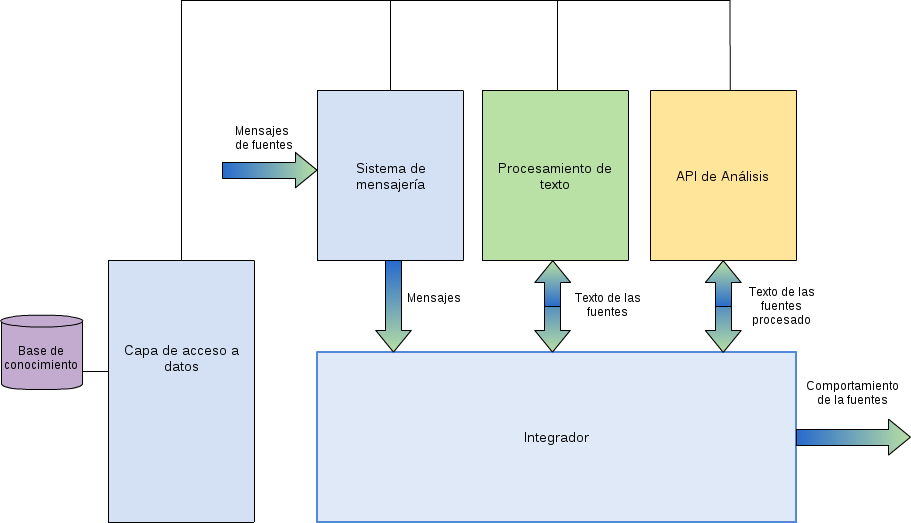
\includegraphics[scale=.5]{images/arquitectura}
  \caption{Arquitectura general del sistema}
  \label{arquitectura}
  \end{center}
\end{figure}
